\documentclass[11pt]{beamer}
\usetheme{Warsaw}
\usepackage[utf8]{inputenc}
\usepackage[english]{babel}
\usepackage{amsmath}
\usepackage{amsfonts}
\usepackage{amssymb}
\usepackage{graphicx}
\usepackage[T1]{fontenc}
\usefonttheme[onlymath]{serif}
\setbeamertemplate{blocks}[rounded][shadow=true]


\author{Sacha GRELET-RIOUT and Hugo BRUHIER}
\title{Cooled Ablation}

%\setbeamercovered{transparent} 
\setbeamertemplate{navigation symbols}{} 
\logo{\includegraphics[width=0.5cm]{Logo_TSE.png}} 
\institute{Télécom Saint-Étienne} 
\date{\today} 
\subject{Physics} 

\addtobeamertemplate{footline}{\insertframenumber/\inserttotalframenumber}

\begin{document}
\setbeamertemplate{caption}{\raggedright\insertcaption\par}

\begin{frame}
\titlepage
\end{frame}

\begin{frame}
\tableofcontents
\end{frame}

\section{Introduction}
\subsection{What is laser ablation ?}
\begin{frame}

\begin{figure}[H]
\centering
\includegraphics[height=160px]{laser_ablation.jpg}
\caption{Laser ablation}
\end{figure}

\end{frame}

\subsection{Principles of cooled laser ablation}
\begin{frame}{The "Toy model"}
\onslide<1->
One pulse instantaneous temperature rise:
$
\Delta T \propto E_p
$
\\
\vspace{15px}
\onslide<2->
Material cools at:
$
\frac{1}{\sqrt{1+t/\tau_0}}
$
\\
\vspace{15px}
\onslide<3->
Temperature of the surface encountered by the (n+1)$^\text{th}$ pulse:
\center{$
T_n+1 = T_n+\delta T
$
 with 
$
\delta T = \frac{\Delta T}{\sqrt{1+\tau_R / \tau_0}}
$}

\end{frame}

\begin{frame}{Ablation after \emph{m} pulses : Proof}

\onslide<1->
$$
T_c < T_{material} = T_0 + \Delta T + \frac{\Delta T}{\sqrt{1+\frac{\tau_R}{\tau_0}}} + \frac{\Delta T}{\sqrt{1+\frac{\tau_R}{\tau_0}}} + ...
$$
\onslide<2->
$$
\Leftrightarrow T_C = T_0 + \Delta T + (m-1) \frac{\Delta T}{\sqrt{1+\frac{\tau_R}{\tau_0}}}
$$
\onslide<3->
$$
\Leftrightarrow T_c = T_0 + \Delta T + (m-1) \delta T
$$
\onslide<4->
$$
\Leftrightarrow m-1 = \frac{T_c - T_0 - \Delta T}{\delta T}
$$
\onslide<5->
$$
\Leftrightarrow \boxed{m = \frac{T_c - T_0 - \Delta T + \delta T}{\delta T}}
$$


\end{frame}


\section{MatLab simulation}

\subsection{Choices of programmation}
\begin{frame}{Why we choose MatLab ?}
\begin{block}{Positive aspects}<+->
\begin{itemize}
\item<+-> Simple to use,
\item<+-> A lot of things are already coded,
\item<+-> A big community is active,
\item<+-> We use it in others courses at Télécom.
\end{itemize}
\end{block}

\begin{block}{Negative aspects}<+->
\begin{itemize}
\item<+-> MatLab is, sometimes, a "black box",
\item<+-> It is not a free software.
\end{itemize}
\end{block}
\end{frame}


\subsection{Results}
\begin{frame}


\begin{figure}[H]
\centering
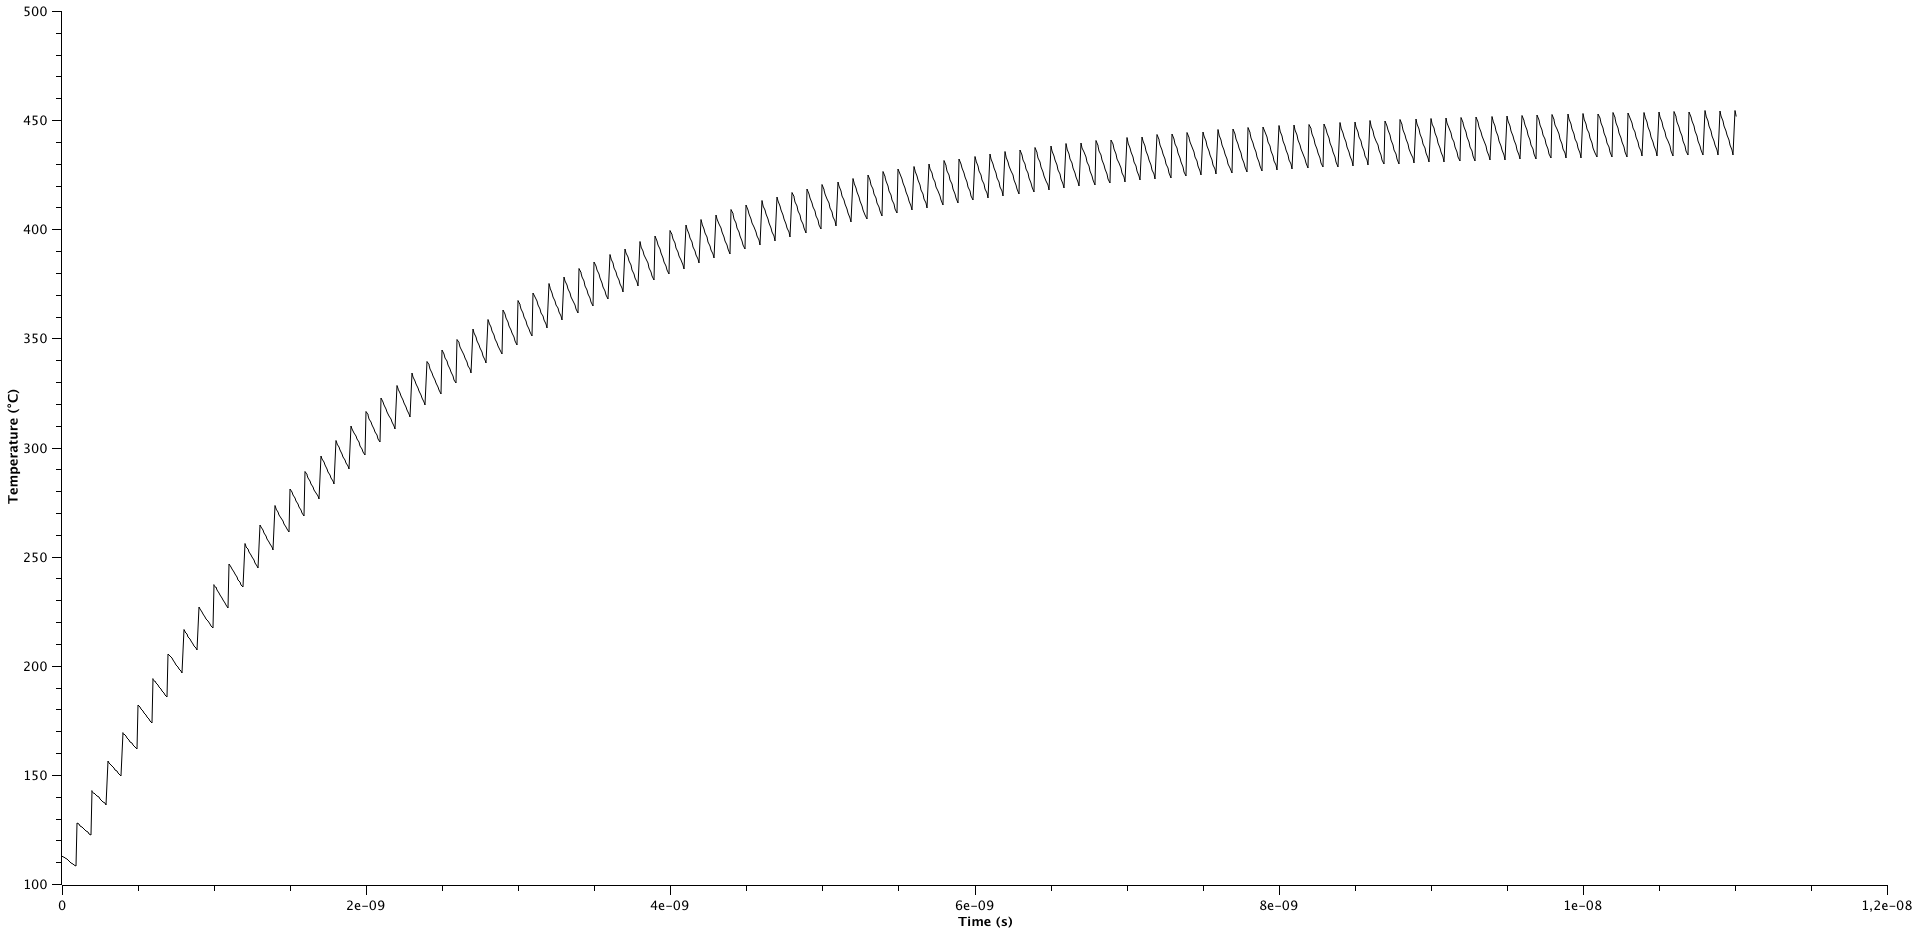
\includegraphics[height=150px]{temperature_evolution_of_the_impact_point.png}
\caption{Temperature evolution of the impact point}
\end{figure}

\end{frame}

\begin{frame}

\begin{figure}[H]
\centering
\includegraphics[height=160px]{temperature_evolution_of_the_impact_point_2.png}
\caption{Differents values of $E_p$ and $\tau_R$}
\end{figure}

\end{frame}

\section{Application of this ablation : Dentin Ablation}
\begin{frame}{What is "Dentin"}

\begin{figure}[H]
\centering
\includegraphics[height=160px]{dentine.png}
\caption{Scheme of the structure of a teeth}
\end{figure}

\end{frame}

\begin{frame}{Dentin Ablation}

\begin{figure}[H]
\centering
\includegraphics[height=150px]{cooling_system.png}
\caption{The cooling system of the dentin ablation}
\end{figure}


\end{frame}

\begin{frame}{Results}

\begin{figure}[H]
\centering
\includegraphics[height=150px]{dentine_impacts.png}
\caption{Ablation of the dentin}
\end{figure}

\end{frame}

\section{Conclusion}

\begin{frame}{Conclusion}
\large
\begin{itemize}
\item Young process which open new applications of laser ablation,
\item Impacts with reduced collateral damages,
\item Low energy of laser,
\item The theory is young and "too" simple.
\end{itemize}
\end{frame}

\section*{Thanks}
\begin{frame}
\center
\huge{Thank you for your attention}
\end{frame}

\begin{frame}{References}

\begin{itemize}
\item "Ablation-cooled material removal with ultrafast bursts of pulses" - Can Kerse, et. al.
\item "Laser ablation of dentin and its medical application" - Quang Tri Le
\end{itemize}

\end{frame}
\end{document}